\subsection{Giao diện khám phá}

Hệ thống cung cấp chức năng khám phá cho phép người dùng khám phá những khía cạnh khác nhau của ảnh như nhãn, vị trí chụp, khuôn mặt trong bức ảnh.

Các nhãn được phân loại từ các ảnh người dùng tải lên sẽ được hệ thống phân loại, nhóm thành các nhóm khác nhau dựa theo địa điểm, hành động và sự kiện trong ảnh như Hình \ref{fig:explore_label}.

\begin{figure}[H]
    \centering
    \begin{subfigure}{0.48\textwidth}
        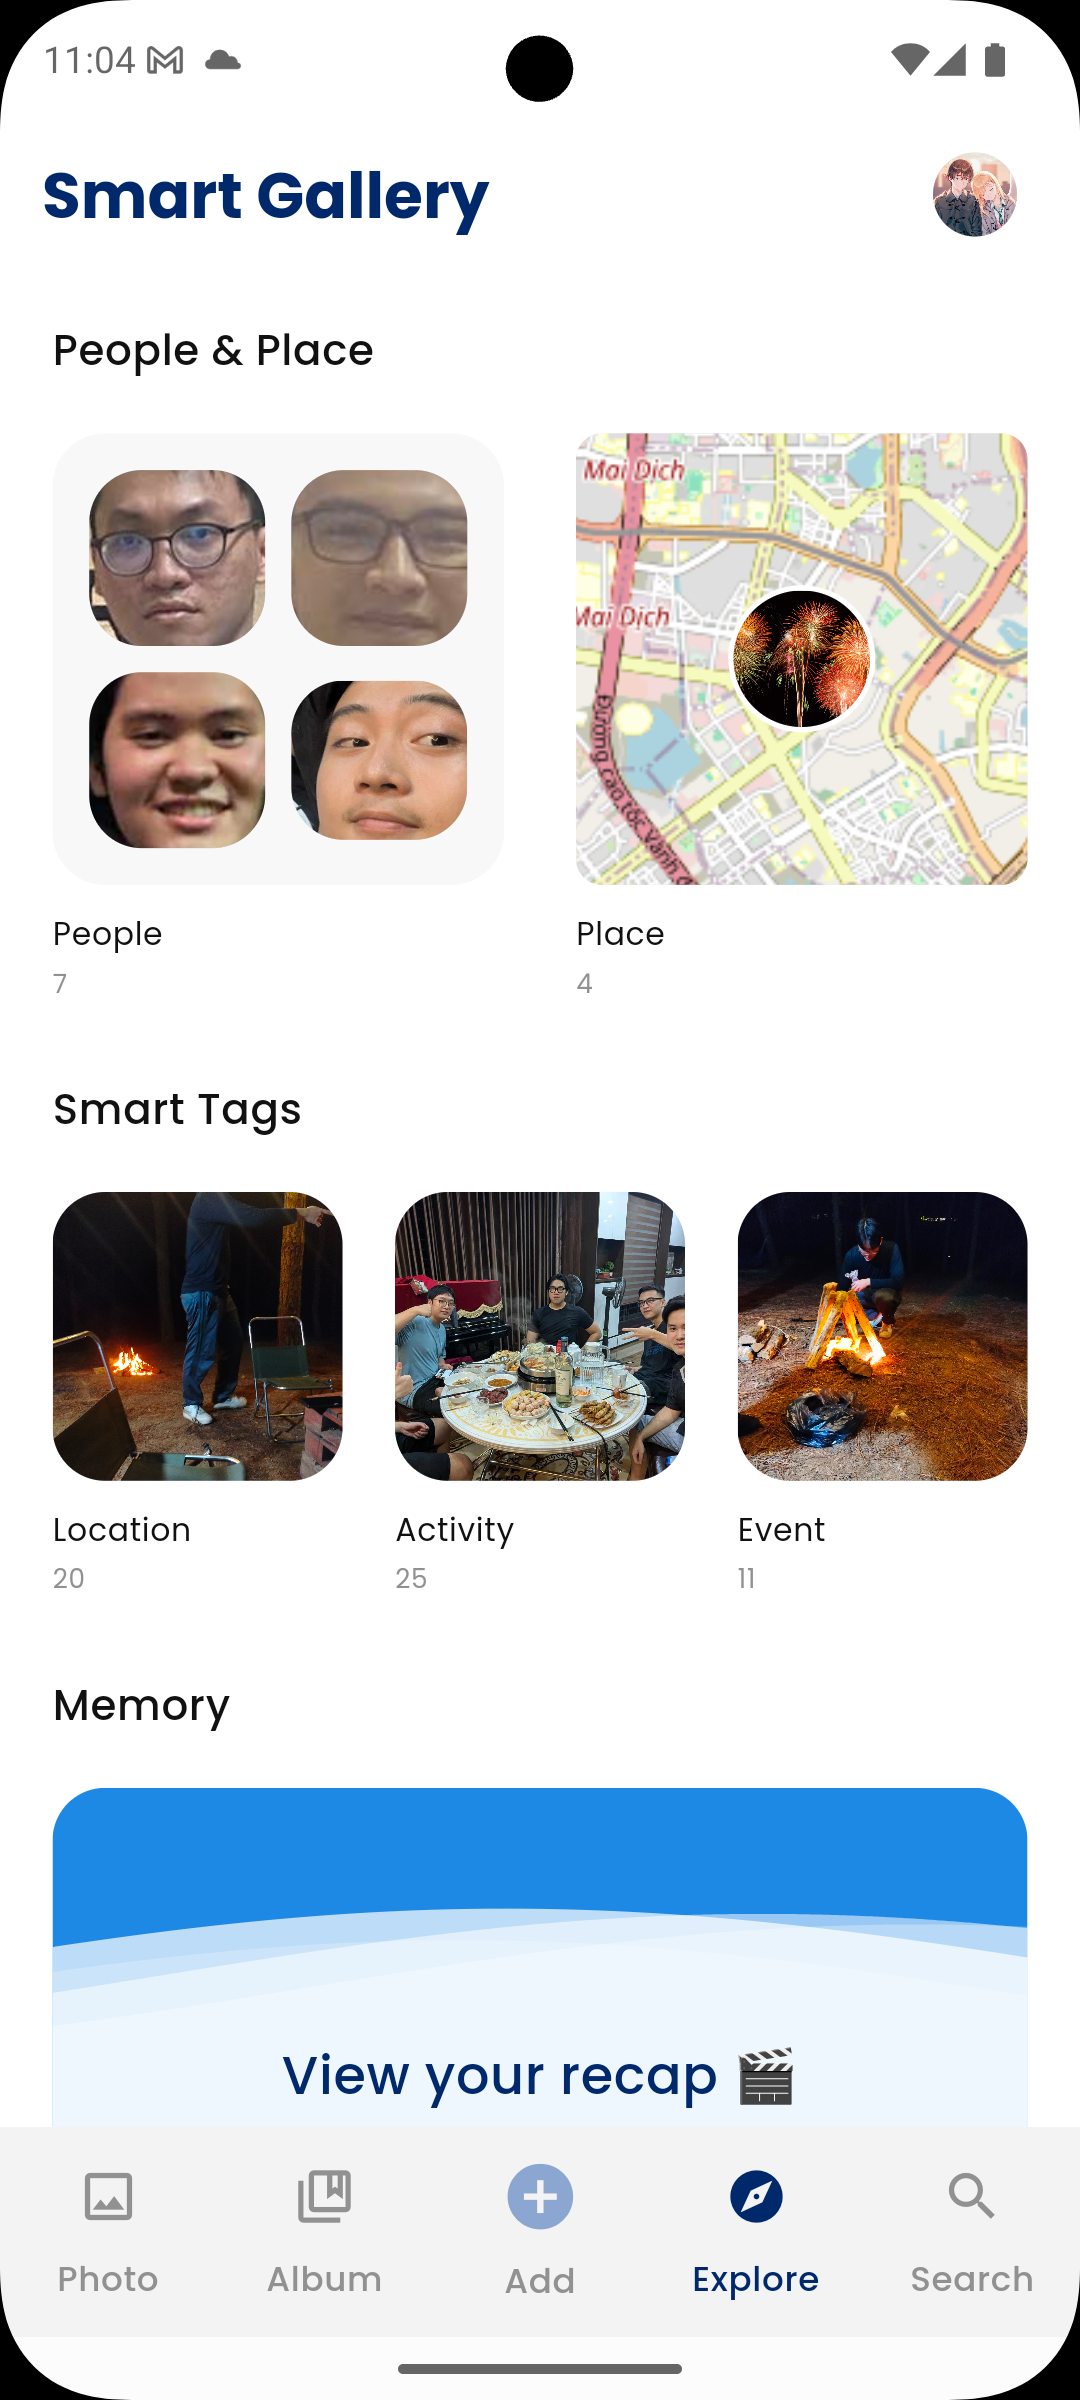
\includegraphics[width=1\linewidth]{figures/c4/4-2/explore_1.png} 
        \caption{Trang chủ}
    \end{subfigure}
    \hfill
    \begin{subfigure}{0.48\textwidth}
        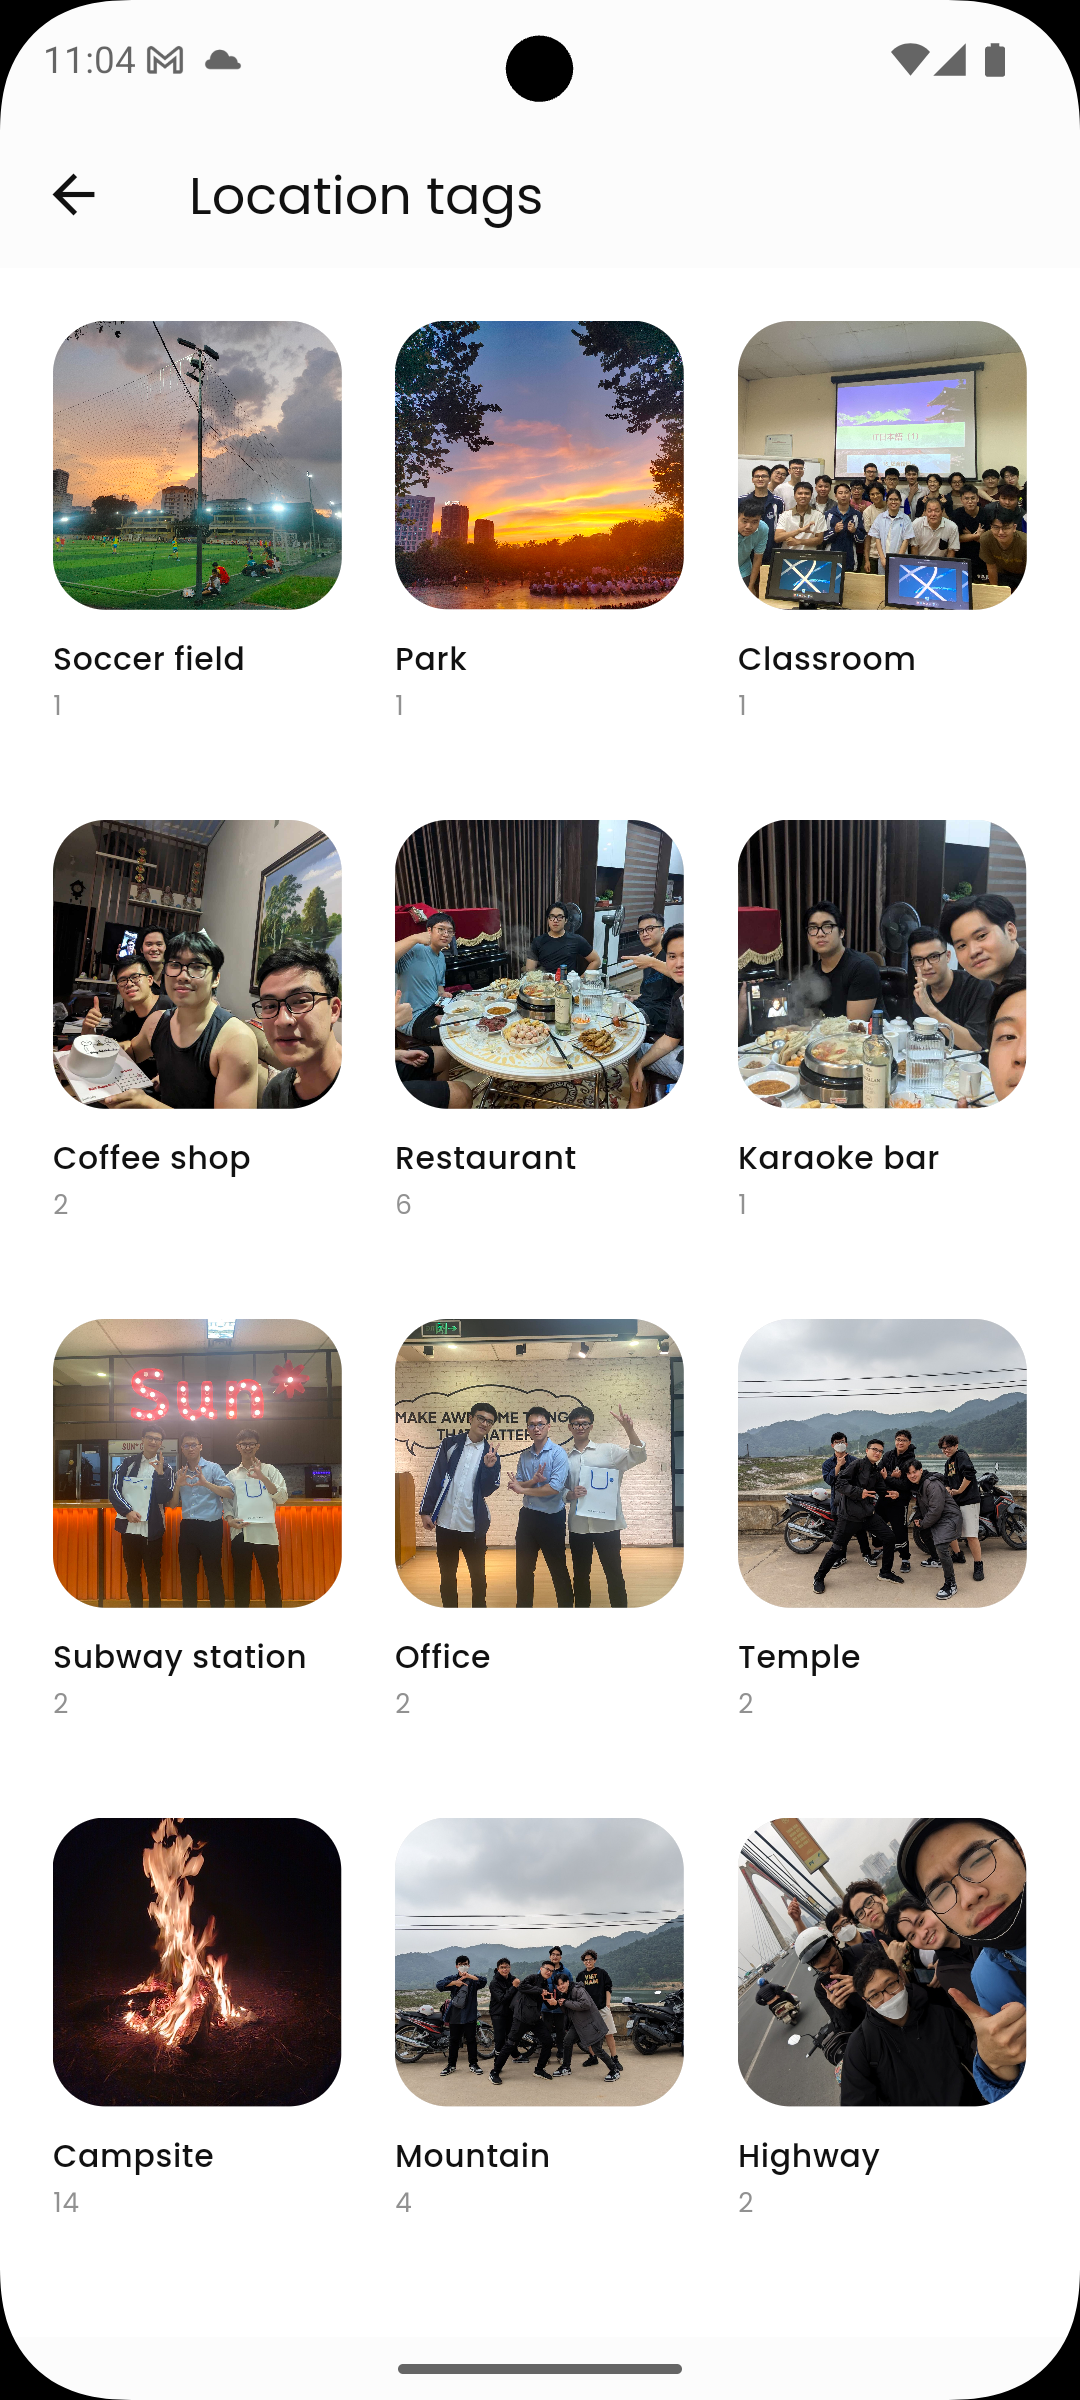
\includegraphics[width=1\linewidth]{figures/c4/4-2/explore_2.png} 
        \caption{Danh sách nhãn ảnh}
    \end{subfigure}
    \caption{Giao diện khám phá.}
    \label{fig:explore_label}
\end{figure}

Hệ thống cũng cung cấp tính năng quản lý ảnh theo địa điểm. Người dùng có thể xem, chỉnh sửa các vị trí cho ảnh, đồng thời được hệ thống phân nhóm các ảnh theo vị trí chụp như Hình \ref{fig:explore_location}.

\begin{figure}[H]
    \centering
    \begin{subfigure}{0.32\textwidth}
        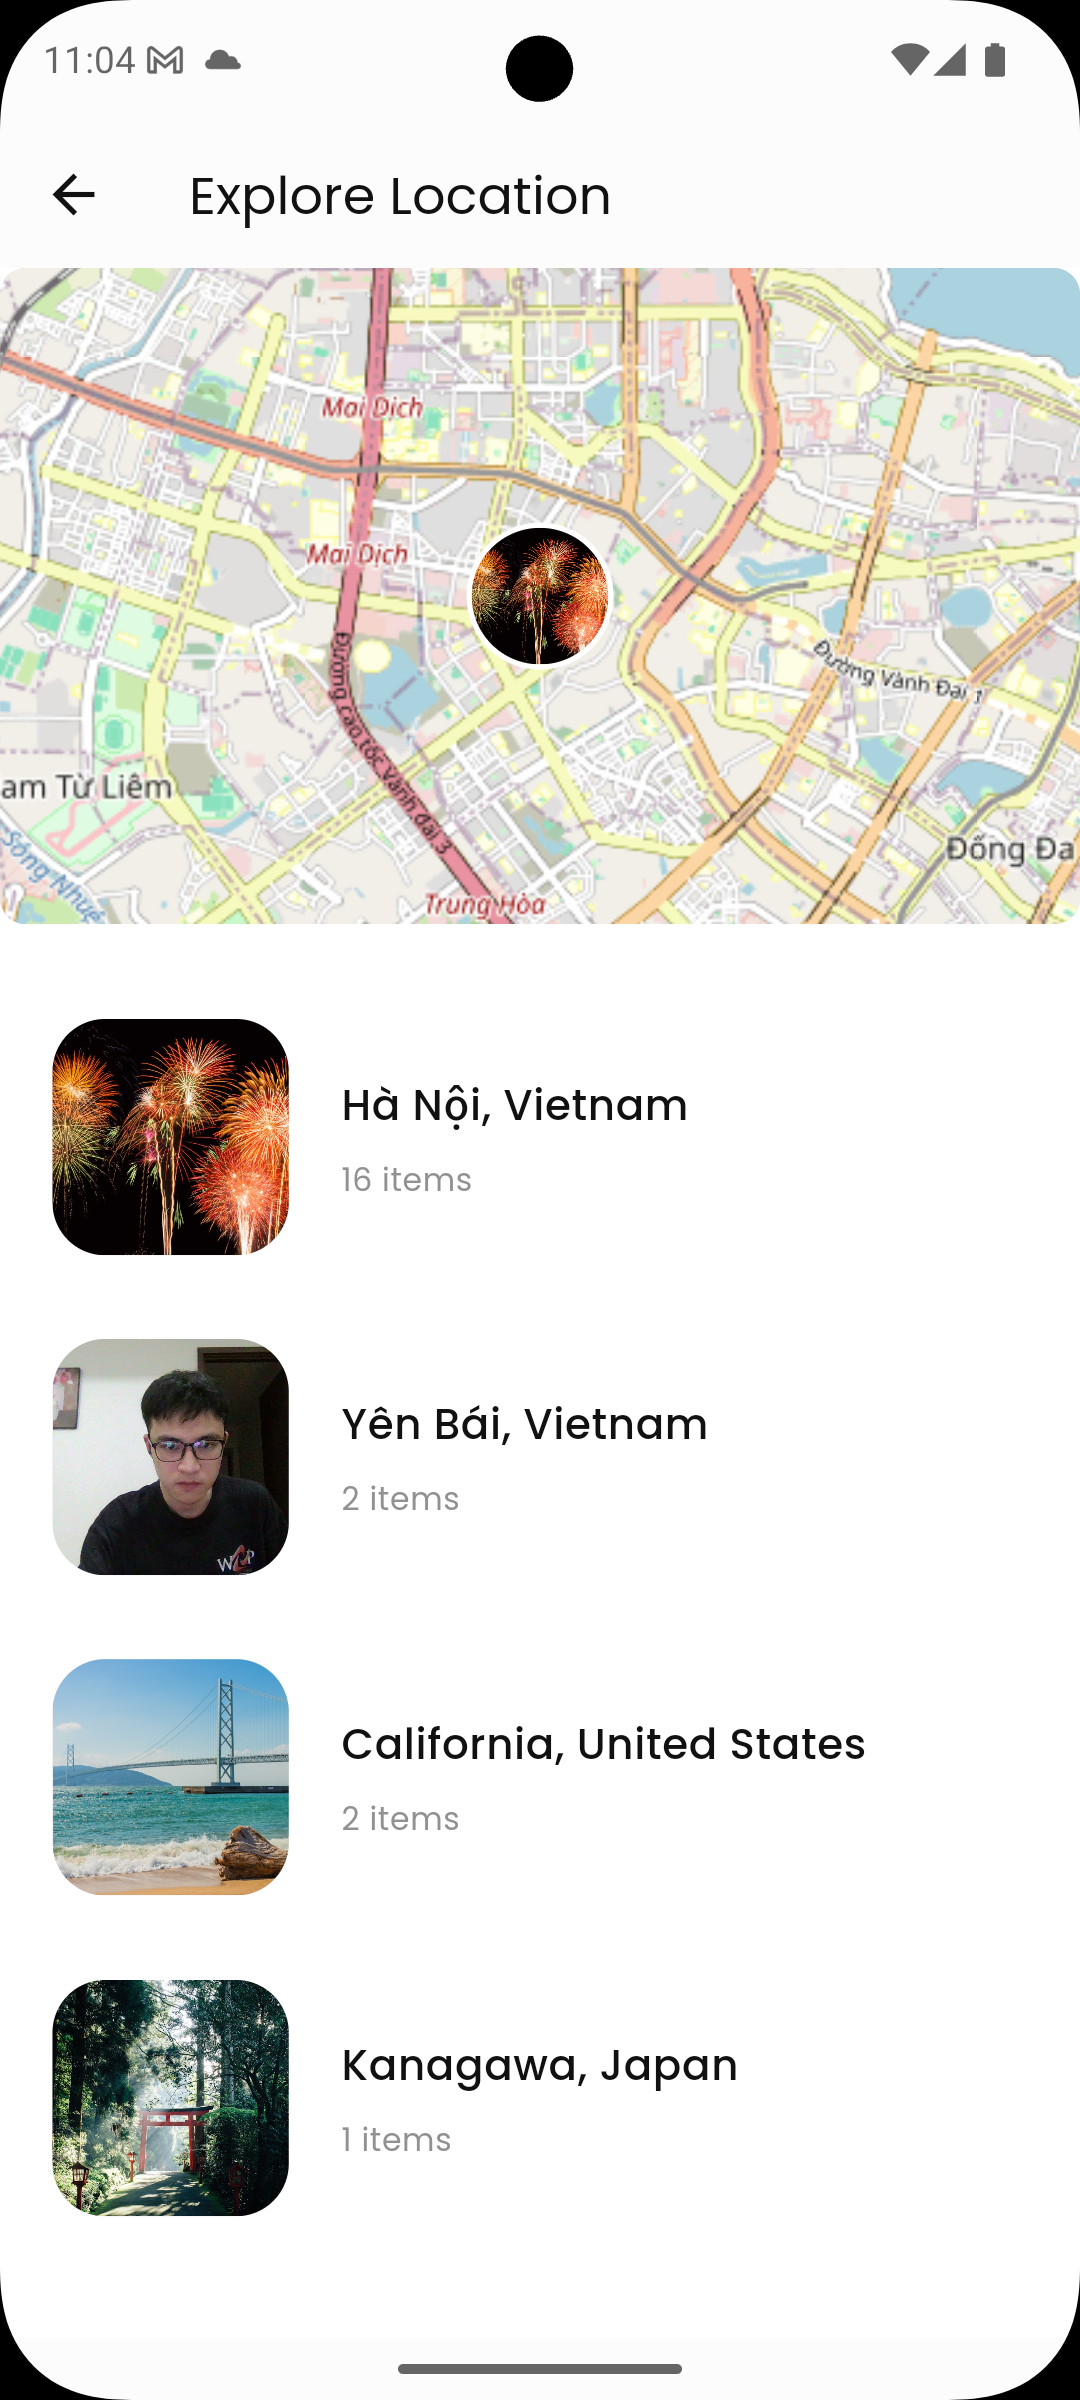
\includegraphics[width=1\linewidth]{figures/c4/4-2/location_1.png} 
        \caption{Nhóm ảnh theo vị trí}
    \end{subfigure}
    \hfill
    \begin{subfigure}{0.32\textwidth}
        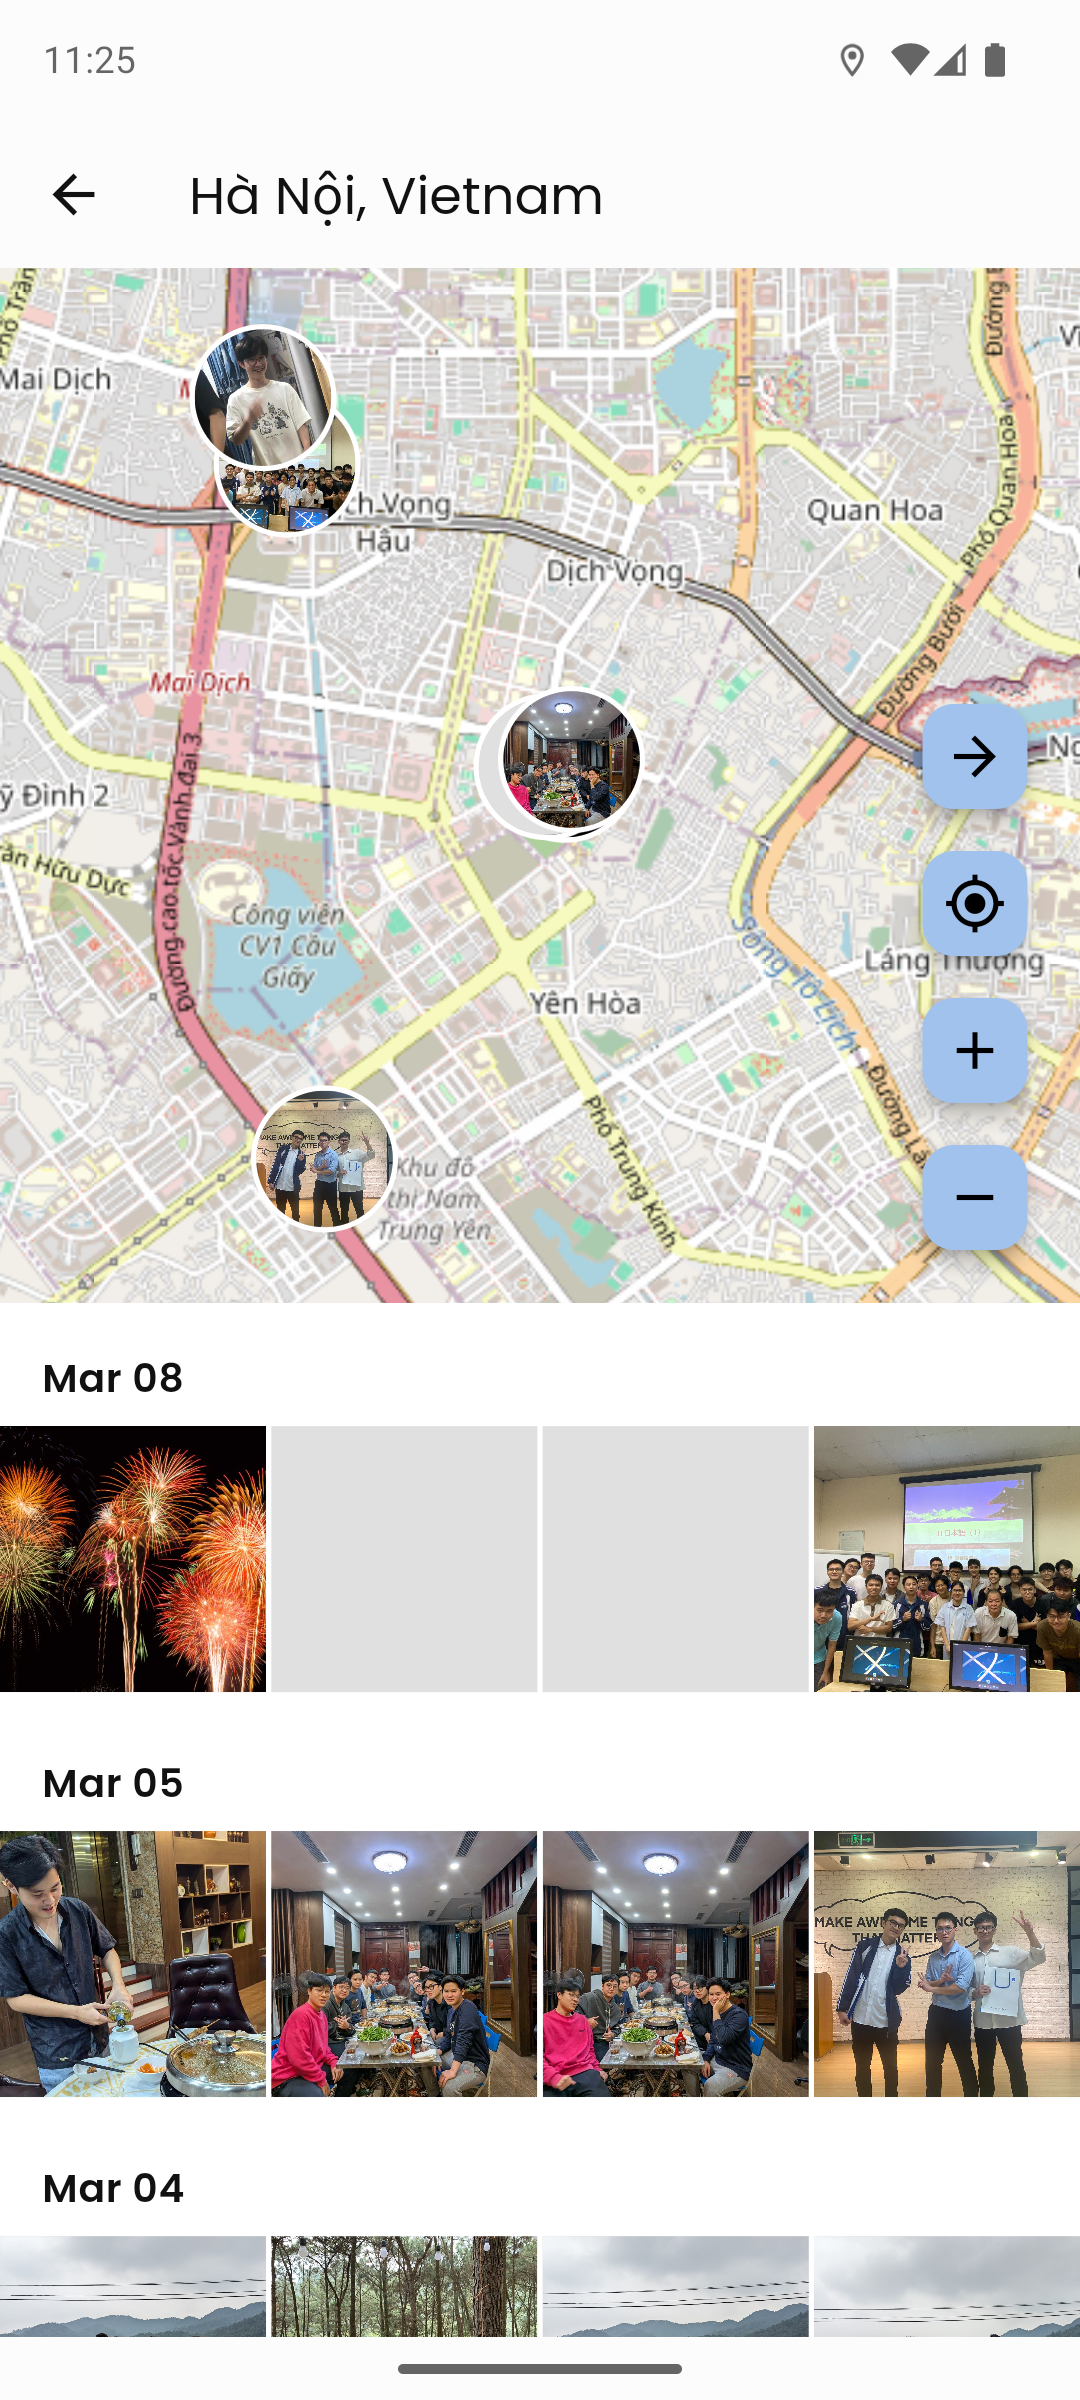
\includegraphics[width=1\linewidth]{figures/c4/4-2/location_2.png} 
        \caption{Xem ảnh theo vị trí}
    \end{subfigure}
    \hfill
    \begin{subfigure}{0.32\textwidth}
        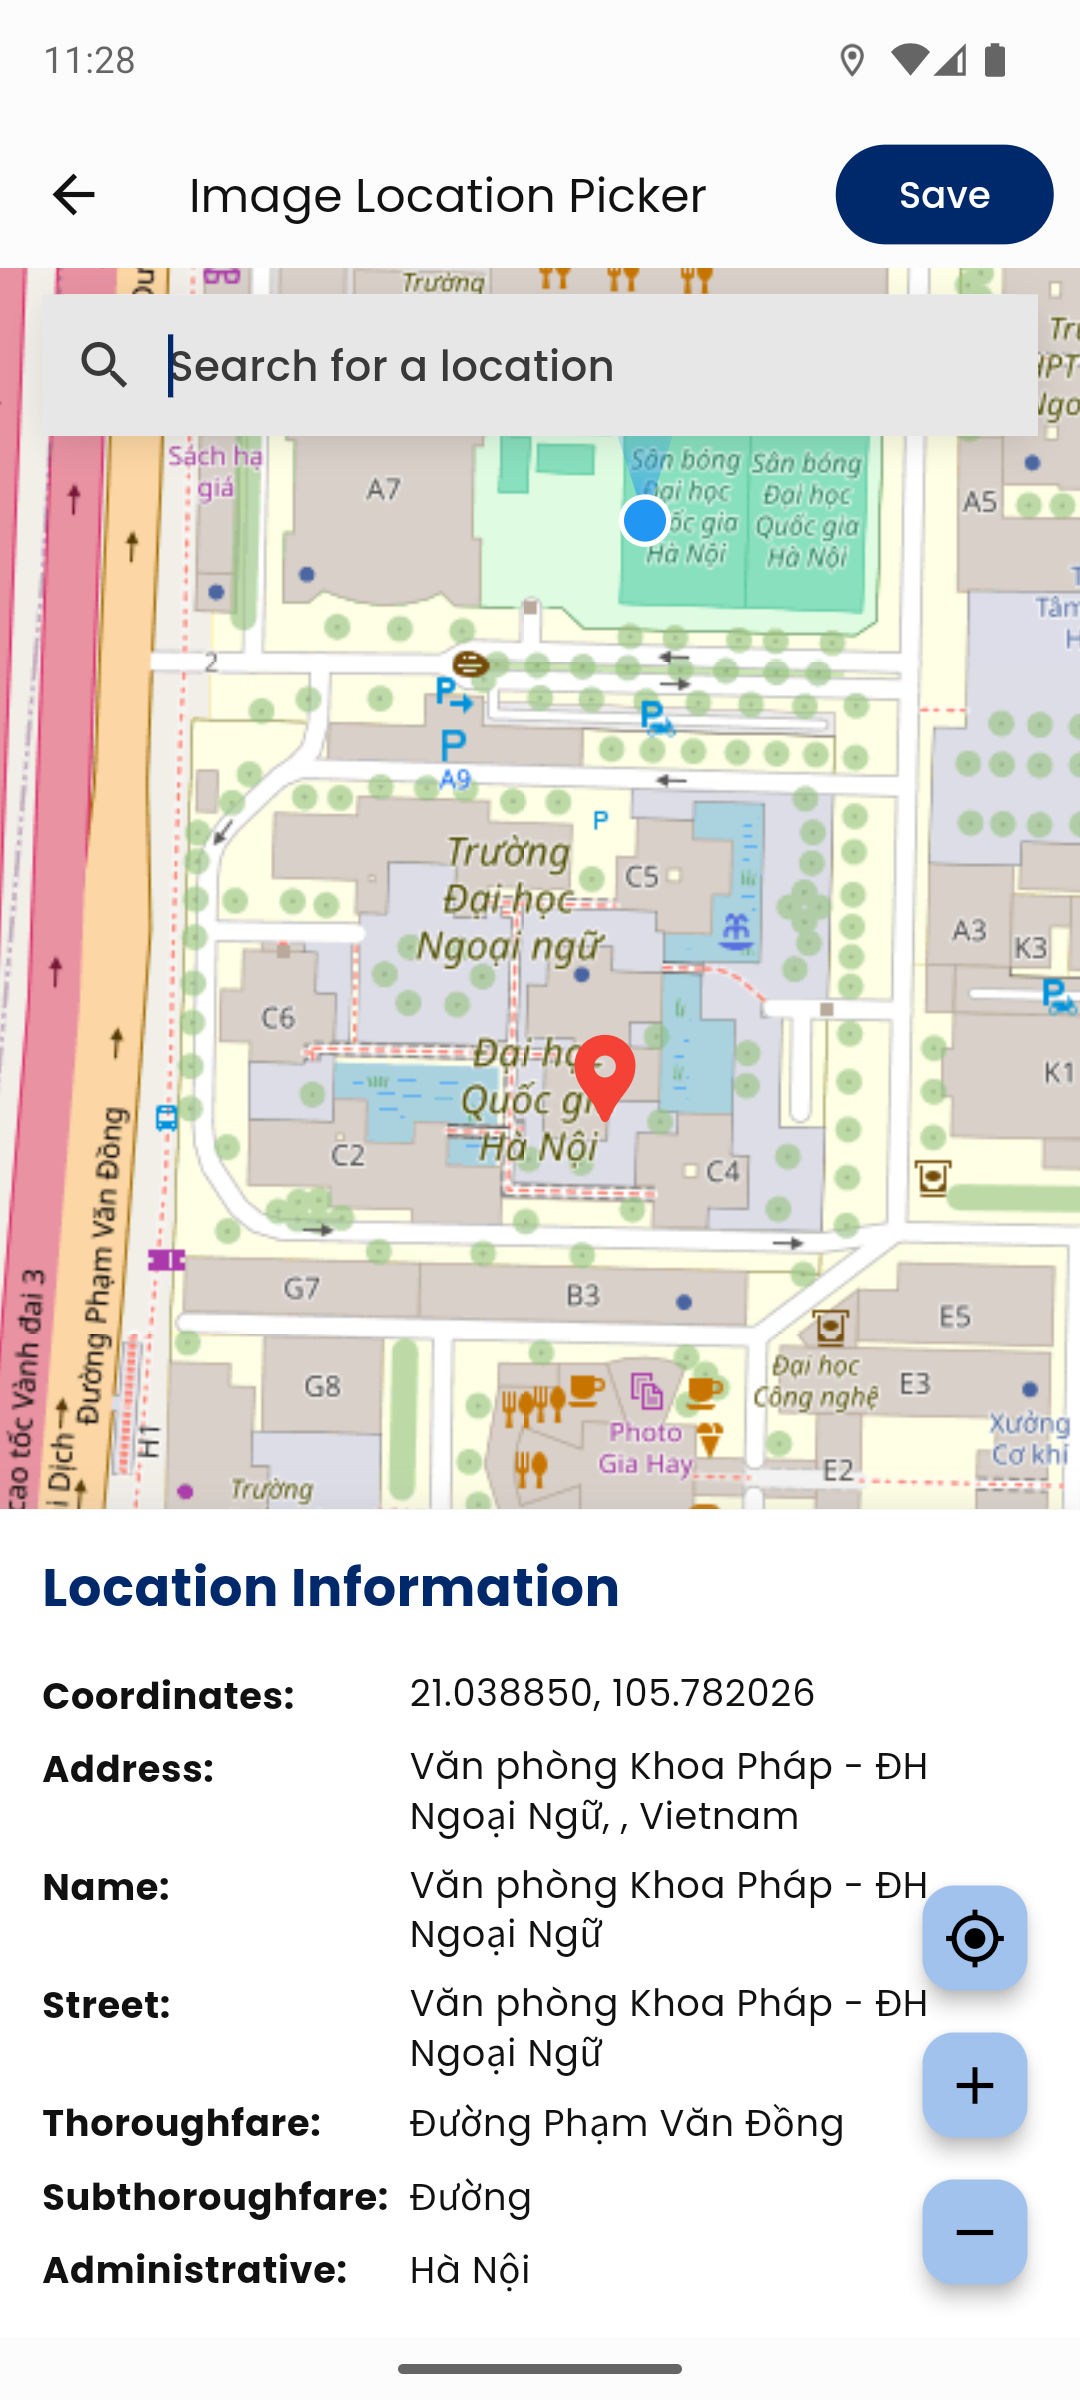
\includegraphics[width=1\linewidth]{figures/c4/4-2/location_3.png} 
        \caption{Thêm vị trí cho ảnh}
    \end{subfigure}
    \caption{Giao diện quản lý vị trí ảnh.}
    \label{fig:explore_location}
\end{figure}

Ngoài ra hệ thống cũng cung cấp tính năng nhận diện khuôn mặt trong ảnh. Người dùng có thể xem, chỉnh sửa các khuôn mặt trong ảnh, đồng thời được hệ thống phân nhóm các ảnh theo khuôn mặt như Hình \ref{fig:explore_face}.

\begin{figure}[H]
    \centering
    \begin{subfigure}{0.48\textwidth}
        
\includegraphics[width=1\linewidth]{figures/c4/4-2/face_1.png} 
        \caption{Danh sách khuôn mặt}
    \end{subfigure}
    \hfill
    \begin{subfigure}{0.48\textwidth}
        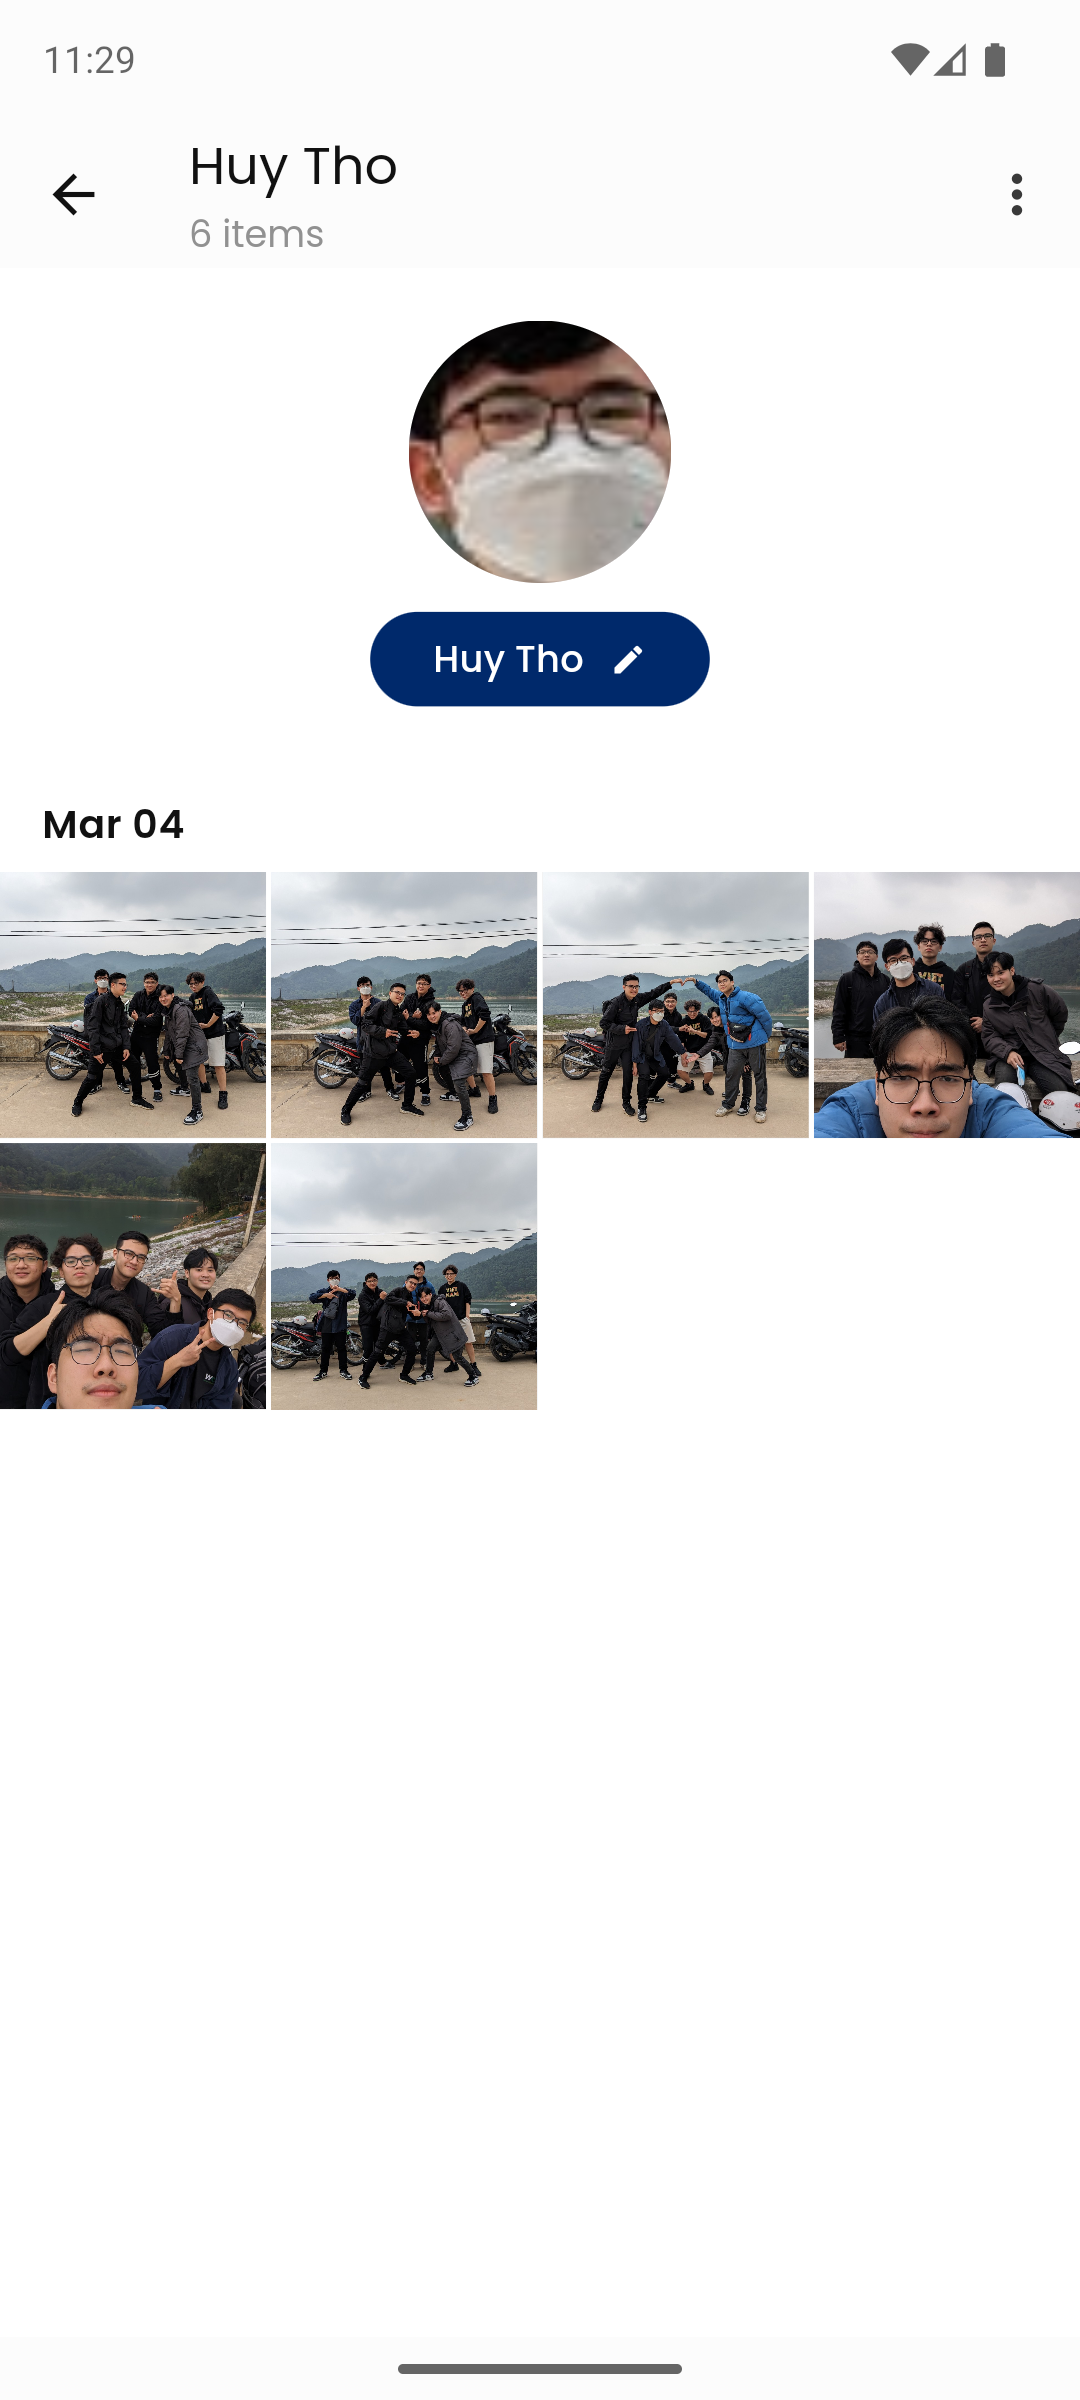
\includegraphics[width=1\linewidth]{figures/c4/4-2/face_2.png} 
        \caption{Xem ảnh theo khuôn mặt}
    \end{subfigure}
    \caption{Giao diện quản lý khuôn mặt.}
    \label{fig:explore_face}
\end{figure}